\documentclass[a4paper,zihao=5]{ctexbeamer}
\usetheme{CambridgeUS}
\usepackage{graphicx}
\usepackage{amsmath}
\usepackage{amssymb}
\usepackage{float}
\usepackage{hyperref}
\providecommand{\keywords}[1]{\\\textbf{\textit{关键词:}}#1}
\title{个人养老金:全球视角与中国特色}
\author{董晨阳\thanks{学号2201211201}\and 李昭伦\thanks{学号2201211203}}
\date{\today}
\begin{document}
\AtBeginSection[]
{
    \small\begin{frame}
        \frametitle{目录}
        \tableofcontents[
            sectionstyle=show/shaded,
            subsectionstyle=show/show/hide,
            subsubsectionstyle=show/show/show/hide
        ]
    \end{frame}
}
\maketitle
\section{个人养老金的全球多样性}
\begin{frame}
    \frametitle{个人养老金政策出台}
    发展个人养老金,是应对人口老龄化压力、完善养老体系的重要改革举措。经过长期论证,我国于2018年启动个人养老金制度建设,2022年加快部署,进展包括:
    \begin{enumerate}
        \item 4月,国务院办公厅发布《关于推动个人养老金发展的意见》;
        \item 6月,人社部、财政部、国家税务总局、银保监会、证监会联合印发《关于推动个人养老金发展的意见》宣传提纲
        \item 6月,证监会发布《个人养老金投资公开募集证券投资基金业务管理暂行规定(征求意见稿)》
        \item 11月个人养老金制度正式启动,北京、上海、广州、西安、成都等36个城市和地区成为“先行者”。
    \end{enumerate}
\end{frame}

\begin{frame}
    \frametitle{养老金资产国内外差异明显}
    分析个人养老金发展前景,确实需要参考海外市场经验,但是分析框架需要升级,不能停留在列举个别案例的层面,而应从全球养老金的多样化实践中寻找普遍规律,以此为基础推导我国乃至全球个人养老金的发展前景,并根据中国具体国情做出修正。
    \begin{figure}[H]
        \begin{minipage}{0.48\linewidth}
            \centering
            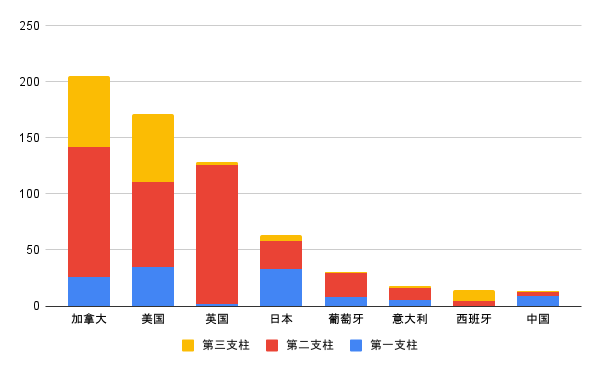
\includegraphics[width=\linewidth]{img/三支柱规模占GDP比重.png}
            \caption{养老储备规模与结构差异明显}
        \end{minipage}
        \begin{minipage}{0.48\linewidth}
            \centering
            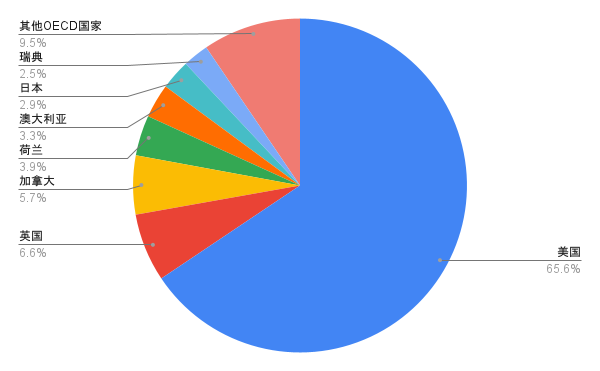
\includegraphics[width=\linewidth]{img/totalOECDpensionassets.png}
            \caption{养老金资产的全球分布极不均匀}
        \end{minipage}
    \end{figure}
\end{frame}

\section{他山之石:海外养老金第三支柱发展经验}
\subsection{美国:第三支柱发展成熟,资产配置以共同基金为主}
\begin{frame}
    \frametitle{美国IRAs:主要来自第二支柱转存}

    第一支柱(联邦社保基金,OASDI)、第二支柱(职业养老金,401(k)等)、第三支柱(个人退休账户,IRAs)分别为2.9万亿美元、20.1万亿美元和12.2万亿美元,占比8\%、57\%和35\%。IRAs资金主要来自第二支柱转存。

    IRAs可投资范围广泛,共同基金占到IRAs资产配置的半壁江山,指数基金和目标日期基金受青睐。
    \begin{figure}[H]
        \begin{minipage}{0.48\linewidth}
            \centering
            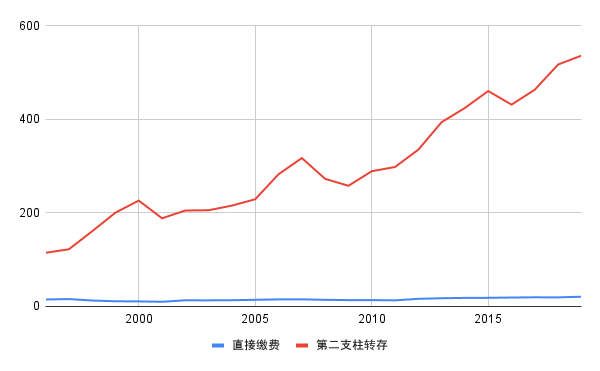
\includegraphics[width=0.8\linewidth]{img/第二支柱转存构成传统型IRA主要资金来源.png}
            \caption{第二支柱转存构成IRA主要资金来源}
        \end{minipage}
        \begin{minipage}{0.48\linewidth}
            \centering
            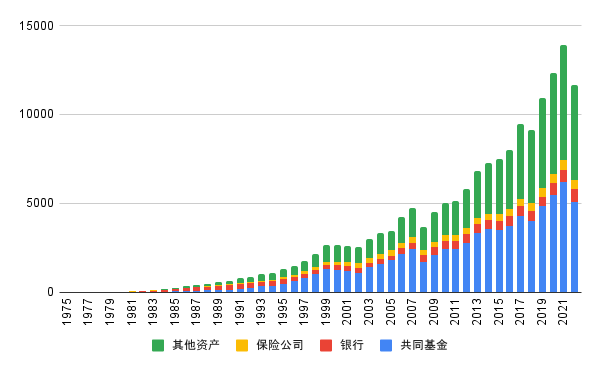
\includegraphics[width=\linewidth]{img/共同基金占据IRAs资产配置的半壁江山.png}
            \caption{共同基金占据IRAs资产配置的半壁江山}
        \end{minipage}
    \end{figure}
\end{frame}


\subsection{日本:第三支柱仍处发展初期,资产配置风险偏好提升}
\begin{frame}
    \frametitle{日本:第三支柱仍处发展初期}
    日本第三支柱实行 iDeCo 和 NISA 双账户制,多层次鼓励居民进行养老储蓄投资。截至2019年末,日本养老金第一、第二和第三支柱(iDeCo、NISA)的资产管理规模分别为157.9万亿、74.6万亿和10.7万亿日元,占比65\%、31\%和4\%。

    iDeCo各类资产配置相对均衡,近年来中高风险资产占比有所提升。NISA资产配置以股票、投资信托为主,风险偏好较高。NISA账户设立目的之一是引导居民由储蓄转向投资,投资范围被限定为股票、投资信托等中高风险资产。
    \begin{figure}[H]
        \centering
        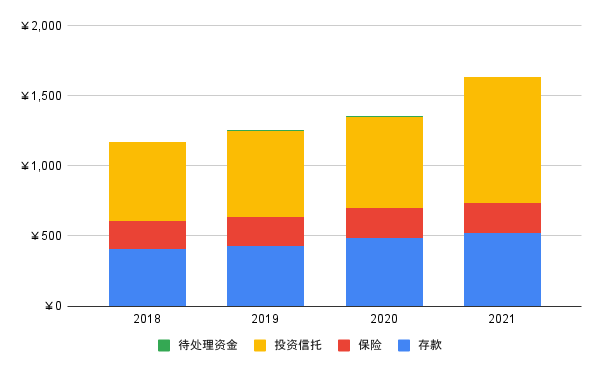
\includegraphics[width=0.5\linewidth]{img/iDeCo投资风险偏好提升.png}
        \caption{iDeCo投资风险偏好提升}
    \end{figure}
    % 截至2020年末,NISA资产余额中股票、投资信托、ETF和REIT分别占比36.2\%、61.4\%、1.5\%和1\%。
\end{frame}




\subsection{德国:第三支柱起补充作用,资产配置以保险产品为主}
\begin{frame}
    \frametitle{德国里斯特计划:起补充作用}
    德国养老金体系以第一支柱为核心,第二、三支柱起补充作用,2019年德国65岁以上老人收入的61\%来自第一支柱,8\%来自第二支柱(企业年金),14\%来自第三支柱(里斯特计划等),其余来自居民储蓄。政府对里斯特计划采用多种形式补贴,促进个人养老金积累。2017年,政府补贴占到里斯特计划保险合同收入的25\%。

    受民众保守的投资偏好和负利率市场环境影响,德国第三支柱资产配置以保险为主。以第三支柱主要的税优账户里斯特计划为例,保险合同一直是其最主要的投资品类。2020年,保险合同占到里斯特计划全部合同的66\%。
    \begin{figure}[H]
        \centering
        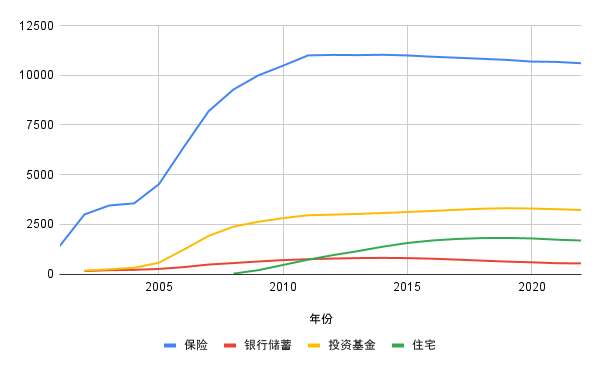
\includegraphics[width=0.5\linewidth]{img/保险合同是里斯特计划最主要投资品类.png}
        \caption{保险合同是里斯特计划最主要投资品类}
    \end{figure}
\end{frame}

\section{个人养老金规模的影响因素}

\subsection{人口特征}
\begin{frame}
    \frametitle{年龄结构与预期寿命}
    \begin{itemize}
        \item 年龄结构变化首先促进养老金积累,然后可能会形成养老金减量压力。在抚养比小于35\%时,个人养老金仍然可以实现较快积累,但平均增速递减。只有当抚养比超过35\%,个人养老金占GDP比重才进入相对稳定状态。
        \item 预期寿命延长则促进养老金积累。在给定退休年龄的前提下,预期寿命延长意味着退休时间相较工作时间得到延长,居民需要在工作阶段积累更多的养老储蓄,用以退休后的消费支出。
    \end{itemize}
    \begin{figure}[H]
        \centering
        \begin{minipage}{0.48\linewidth}
            \centering
            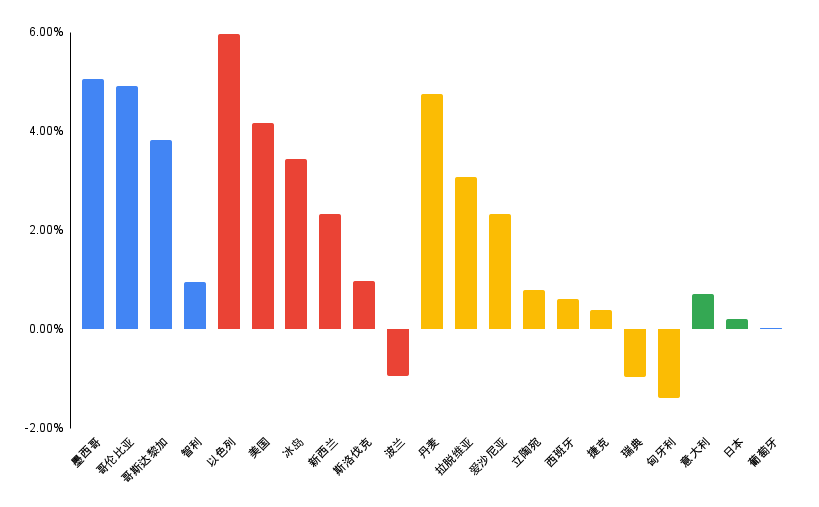
\includegraphics[width=\linewidth]{img/随着老年付养比提高,养老金积累增速开始下降.png}
            \caption{从左到右颜色对应老年抚养比0-20\%,20-30\%,30-35\%,35\%以上}
        \end{minipage}
        \begin{minipage}{0.48\linewidth}
            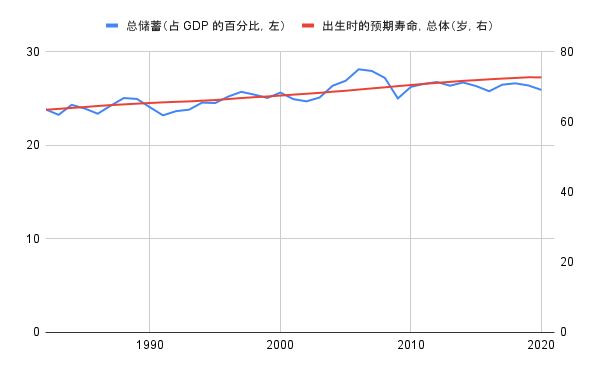
\includegraphics[width=\linewidth]{img/人口预期寿命与储蓄占GDP比重同步上升.png}
            \caption{预期寿命与储蓄占GDP比重同步上升}
        \end{minipage}
    \end{figure}

\end{frame}

\subsection{经济基础}

\begin{frame}
    \frametitle{经济基础:收入水平、资产配置结构与投资收益率}
    \begin{itemize}
        \item 个人养老金是一种储蓄,而收入水平是影响储蓄的关键因素。
        \item 个人养老金也与居民资产配置结构相关。以住房为代表的部分实物资产同时具备“实物”和“金融”双重属性,如果“金融”属性被放大,则会对个人养老金等其它金融资产形成挤出效应。
        \item 投资收益率提高,可以促进个人养老金积累。高收益率可能会吸引个人投资者减少当期消费、增加储蓄,并提升个人养老金相较其它个人储蓄的吸引力。
    \end{itemize}
    \begin{figure}[H]
        \centering
        \begin{minipage}{0.48\linewidth}
            \centering
            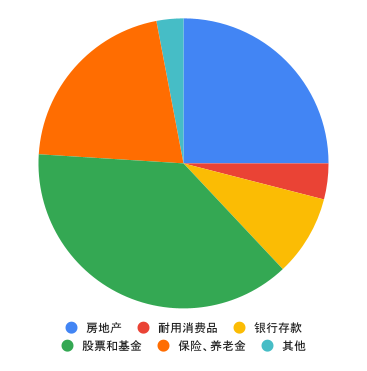
\includegraphics[width=0.75\linewidth]{img/us.png}
            \caption{美国居民资产中房产占比仅约25\%}
        \end{minipage}
        \begin{minipage}{0.48\linewidth}
            \centering
            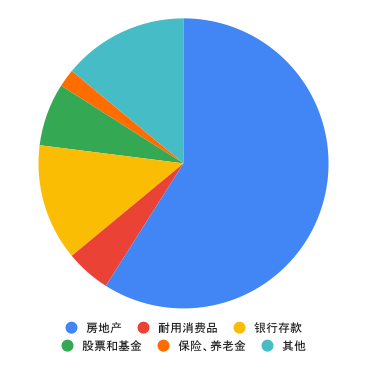
\includegraphics[width=0.75\linewidth]{img/cn.png}
            \caption{中国居民资产中房产占比接近60\%}
        \end{minipage}
    \end{figure}

\end{frame}

% \begin{figure}[H]
%     \centering
%     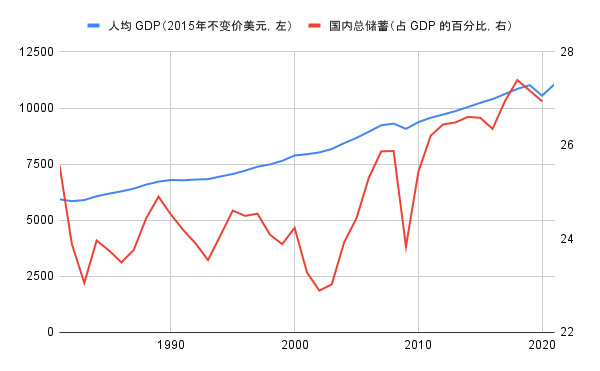
\includegraphics[width=\linewidth]{img/人均收入上升会提升储蓄率.png}
%     \caption{人均收入上升会提升储蓄率}
% \end{figure}




% \begin{figure}[H]
%     \centering
%     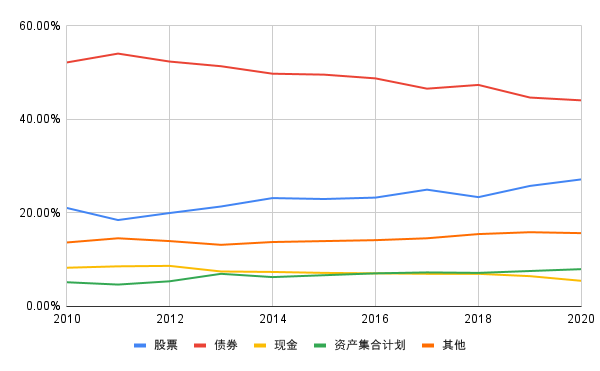
\includegraphics[width=\linewidth]{img/OECD国家私人养老金资产配置中股票占比不断上升.png}
%     \caption{OECD国家私人养老金资产配置中股票占比不断上升}
% \end{figure}

\subsection{制度设计}
\begin{frame}
    \frametitle{制度设计:第一二支柱与税优政策}
    \begin{itemize}
        \item 个人养老金发展规模与公共养老金的支出规模存在较强的负相关关系,反映二者的替代效应。如果公共养老金支出规模较大,势必需要政府财政或居民缴费的支撑,在此背景下居民当期可支配收入减少,降低了于私人储蓄。与此同时,公共养老金支出较高,一般替代率水平也比较高,已经可以满足大部分居民的养老需求,积累私人养老金的必要性下降。
        \item 个人养老金和企业养老金同属于私人养老金,总体来看二者的发展具有正相关性。促进个人养老金发展的关键机制设计在于转化机制。如果没有相互转化机制,由于企业年金更具优势,往往个人养老金发展相对缓慢;而如果存在相互转化机制,个人养老金一般能获得更好发展。
        \item 税优制度也对个人养老金有一定的促进作用。目前世界上主流的免税激励模式是EET型,即在缴费和资本利得阶段享受税收优惠,在提取阶段需要偿还税收优惠。
    \end{itemize}
\end{frame}

\section{中国特色}
\subsection{个人养老金政策与产品现状}
\begin{frame}
    \frametitle{养老金政策的主要特征}
    \begin{enumerate}
        \item 参与主体覆盖面广,参与自由。我国三支柱个人账户允许在中国境内参加一支柱养老保险的全体劳动者参与,第一支柱养老保险当前已覆盖约10亿人口。相比之下,第二支柱参保前提为供职企业设立企业年金,故三支柱养老覆盖面更广,参与更加自由。这一制度设计与美国IRA账户思路基本一致。
        \item 出资与主体:自愿开立,个人出资,个人管理。第三支柱养老体系完全由个人出资,采用完全积累制。不同于第一支柱与第二支柱的统一专户委托管理,第三支柱资金由个人作为投资决策主体。我国试点政策缴纳额度上限最高为12000元,占当年平均工资百分比16.2\%,高于IRA的13.1\%,但低于DC计划38.4\%,符合三支柱特征。
        \item 账户投资范围:投资自由度相对前两支柱较高。个人自主选择购买符合规定的储蓄存款、理财产品、商业养老保险、公募基金等金融产品。考虑到投资者教育水平等因素,我国相较于美国IRA账户投资自由度更低。
        \item 账户开立:养老资金账户仅能在商业银行开立,其他符合规定的金融产品销售机构可代销养老主题金融产品,商业银行把握资金入口,而美国无相关限制。
        \item 资金提取:有待进一步细化。参加人达到领取基本养老金年龄、完全丧失劳动能力、出国(境)定居等经信息平台核验领取条件后,可以按月、分次或者一次性领取个人养老金,领取方式一经确定不得更改,暂未规定强制提取年龄,也未明确提前支取的惩罚性条款。
    \end{enumerate}
\end{frame}

\begin{frame}
    \frametitle{个人养老金产品}

    \begin{enumerate}
        \item 个人养老储蓄:首批23家商业银行发行的储蓄存款(包括4家国有大行发行的特定养老储蓄)
        \item 个人养老金理财产品:包括养老理财产品及其他理财产品,已纳入养老理财试点的11家理财公司可以参与,需要将拟参与个人养老金运行的理财产品报送银保监会。
        \item 个人养老金保险产品:包括年金保险、两全保险,以及银保监会认定的其他产品。目前包括6家机构的7只专属商业养老保险产品。
        \item 个人养老金公募基金:试行阶段,优先纳入养老目标基金,后续适时逐步纳入其他基金。目前包括40家公募机构的129只养老目标基金。
    \end{enumerate}

\end{frame}


\subsection{三支柱养老布局展望}
\begin{frame}
    \frametitle{三支柱养老发展空间广阔}
    \begin{itemize}
        \item 居民收入持续提升有助于提升潜在账户持有率
        \item 人口老龄化深化演进唤醒居民养老意识,提升账户持有意愿
        \item 我国居民在养老金融上风险偏好低、对于银行系产品参与意愿更高
    \end{itemize}
    \begin{figure}[H]
        \begin{minipage}{0.48\linewidth}
            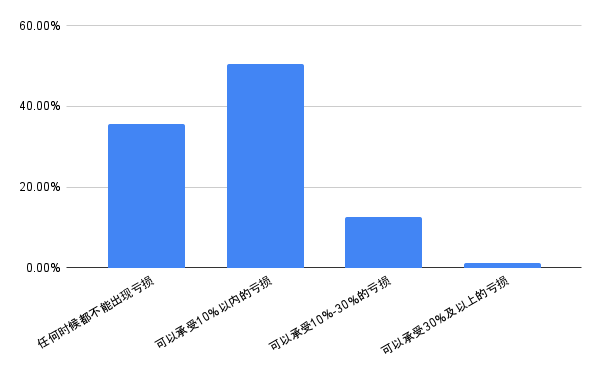
\includegraphics[width=\linewidth]{img/36调查对象无法承受任何亏损.png}
            \caption{36\%调查对象无法承受任何亏损}
        \end{minipage}
        \begin{minipage}{0.48\linewidth}
            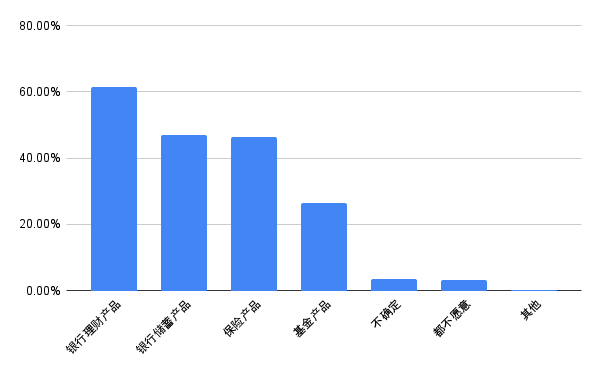
\includegraphics[width=\linewidth]{img/居民对于养老理财、养老储蓄及养老保险参与意愿更高.png}
            \caption{居民对于养老理财、养老储蓄及养老保险参与意愿更高}
        \end{minipage}
    \end{figure}

\end{frame}
\begin{frame}
    \frametitle{产品配置中权益比重有望提升}

    % 2022年中国个人养老金中权益资产比重可能逐步提升至20\%左右,为股票市场提供增量资金约为2000~6000亿元。长期资金流入,有利于提升A股市场机构投资者占比,培养资本市场价值投资与长期投资理念,降低市场波动率,助力资本市场高质量发展。

    % 投资属性上看,商业养老保险具有保本属性、养老理财风险较低、养老基金风险和波动更高;服务属性上看,商业养老保险具备相对优势。养老金融产品包括投资属性和服务属性,从投资属性上看,商业养老保险采取保本+浮动收益,适合风险偏好较低的投资者。养老理财和养老基金均为非保本产品,其中养老理财整体投资期限更长、具有较高的业绩比较基准、产品费率低,同时具有风险保障机制以平滑波动,适合中低风险偏好的投资者;养老基金业绩比较基准以相对收益为主,费率更高,对应风险和收益更高,适合中风险及中高风险投资偏好人群。从服务属性上看,保险产品可附加康养等服务,未来将成为其差异化的竞争点。

    短期而言,渠道端将自上而下影响产品配置。早期银行渠道较为强势,同时,居民风险偏好较低,相较于养老基金等风险较高的产品,储蓄和理财产品在风险程度上与我国养老人群更匹配;此外,养老理财凭借较高的业绩标准、低于其他养老金融产品的费率以及风险保障机制平滑基金波动等优势亦具备较强的吸引力。

    长期而言,底层资产收益率将自下而上影响产品配置。伴随着市场利率下行,以及权益市场向好,养老基金将具备更高的收益和更强的吸引力。长期而言,银行产品的市场份额将部分分流至保险及基金产品,其中,保险产品以其保本+投资的属性将部分替代银行产品的保本功能,而基金产品以相对较高的回报率将部分替代银行产品的收益功能。
    \begin{figure}[H]
        \centering
        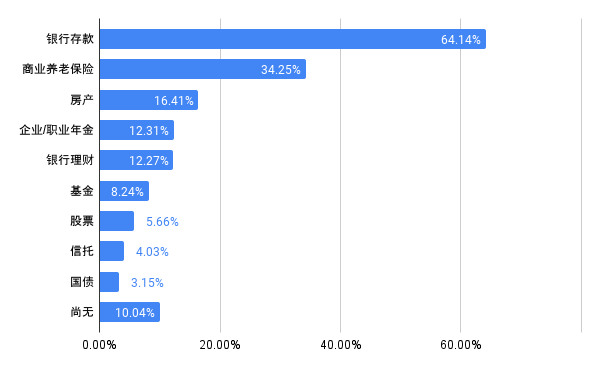
\includegraphics[width=0.5\linewidth]{img/chart.png}
        \caption{银行存款为养老金融最主要的产品途径}
    \end{figure}
\end{frame}


% \section{结论}
% 中国养老体系发展较快但仍相对薄弱,三支柱总量规模仍显不足。虽然我国的财政实力(增加财政用于社保的支出)及保障储备(划转国资充实社保)都可以作为居民养老的潜在补充,但是这些并不能替代三支柱体系。未来第一支柱的扩大可能受制于缴费率和人口老龄化问题。在缴费率难以进一步提升,养老支出在老龄化趋势下可能增加的背景下,第一支柱的规模较难扩大,甚至面临财务持续性问题。因此,在第一支柱扩容可能受限的背景下,我国第二、三支柱(补充养老保险)发展对于我国养老金体系保障能力的提升具有重要意义。

% 海外国家个人养老金的资产配置模式可为我国未来个人养老金的发展提供参考借鉴。虽然我国个人养老金仍处于起步阶段,缺乏相关资产配置比例数据,但如果以企业年金投资状况作为参考,养老投资市场整体风格仍然比较保守。截至2020年底,我国企业年金所推出的养老产品中,权益类养老产品期末资产净值仅占比8\%,呈现比较突出的绝对收益风格,与海外个人养老金平均27.1\%的股票配置比例存在较大差距。面临未来低利率的投资环境,未来我国可能逐步提高养老金对权益类资产的投资比重,以增强投资收益能力和个人养老产品的吸引力,逐渐缩小与海外国家(私人)养老金资产配置结构的差异。

% 个人养老制度的设立可以提高从个人层面对养老资金的多元化投资。这有助于促进资本市场引入新的长期投资者、资产管理机构的发展,以及金融产品的丰富,有助于加速居民资产配置由不动产与存款向金融资产转移,为资本市场带来新类型长期资金。当前我国居民资产配置结构中房产占比接近60\%,相比较美国居民资产配置结构中房产占比不到25\%。发展个人养老制度,也有助于改善中国居民家庭资产配置结构,资本市场有望引入新类型长期投资者。

% \clearpage
% \appendix
% \nocite{*}
% \printbibliography[heading=bibliography]
\end{document}
